\documentclass[11pt,letterpaper]{article}
% ============================================================================
%  한국어판 — XeLaTeX(tectonic) 컴파일. xeCJK + 한글 명조 폰트.
% ============================================================================
\usepackage[margin=1in]{geometry}
\usepackage{amsmath, amssymb, amsthm, amsfonts}
\usepackage{graphicx}
\usepackage{xcolor}
\usepackage{hyperref}
\usepackage{booktabs}
\usepackage{titlesec}
\usepackage{tcolorbox}
\usepackage{fontspec}
\usepackage{xeCJK}
\xeCJKsetup{CJKspace=true}   % 한국어 띄어쓰기(어절 공백) 보존
\setCJKmainfont{AppleMyungjo}
\graphicspath{{../figures/}}
% 캡션/목차 라벨 한글화
\renewcommand{\tablename}{표}
\renewcommand{\figurename}{그림}
\renewcommand{\contentsname}{목차}
\renewcommand{\refname}{참고문헌}
\renewcommand{\abstractname}{초록}
% --- Color Palette ---
\definecolor{ajpblue}{RGB}{28, 54, 115}
\definecolor{ajpsec}{RGB}{54, 95, 145}
\definecolor{bglight}{RGB}{245, 247, 250}
\hypersetup{colorlinks=true, linkcolor=ajpblue, citecolor=ajpsec, urlcolor=ajpblue}
\titleformat{\section}{\large\bfseries\color{ajpblue}}{\thesection}{1em}{}[{\titlerule[0.5pt]}]
\titleformat{\subsection}{\normalsize\bfseries\color{ajpsec}}{\thesubsection}{1em}{}
\newtcolorbox{equationbreakdown}[1]{colback=bglight, colframe=ajpblue,
  fonttitle=\bfseries, title={#1}, arc=3pt, boxrule=1pt, bottomtitle=2mm, toptitle=2mm}
\newtcolorbox{physicsinsight}{colback=bglight, colframe=ajpsec, boxrule=0.5pt,
  left=4mm, right=4mm, top=3mm, bottom=3mm, arc=2pt}
% --- Title & Metadata ---
\title{\vspace{-1.5in}
\rule{\linewidth}{1.5pt} \\ \vspace{4mm}
\large\textbf{일반물리 팀 프로젝트 보고서} \\ \vspace{2mm}
\Large\textbf{문이 쾅 닫힐 때의 회전·마찰 동역학}
\\ \vspace{4mm}
\large\textit{Klein et al., American Journal of Physics 85, 30 (2017) 분석} \\
\rule{\linewidth}{1.5pt}}
\author{
\begin{tabular}{r @{\quad} l}
\textbf{팀:} & Team solvE \,(Group 14) \\[1ex]
\textbf{팀원:} & 채은우 \textit{(데이터 분석, GitHub, 보고서 \LaTeX)} \\
 & 강성민 \textit{(보고서, 시뮬레이션)} \\
 & 장민석 \textit{(실험)} \\
 & 주솔비 \textit{(발표, 영상)} \\[1ex]
\textbf{과목:}  & 일반물리 \\
\textbf{담당교수:}    & Deniz Olgu Devecio\u{g}lu \\
\textbf{소속:}    & DGIST
\end{tabular}}
\date{\today}

\begin{document}
\maketitle
\begin{abstract}
문이 쾅 닫히는 현상은 여러 마찰 메커니즘이 동시에 작용할 수 있는 감쇠 회전운동의 간단한
예이다. Klein 등은 마찰 토크의 세 가지 표준적인 속도 의존성, 즉 일정(건마찰), 1차
(스토크스), 2차(뉴턴 공기저항) 중 어느 것이 운동을 가장 잘 기술하는지를 조사하였다. 본
보고서는 이들의 분석을 이론과 실험 양면에서 재현한다. 실제 문의 각속도를 스마트폰
자이로스코프로 직접 측정하여, 원논문에서 사용한 반경방향 가속도로부터의 환산 과정을 거치지
않았다. 서로 다른 초기 각속도의 두 슬램을 측정하고, 각각의 자유회전 구간에 6개 마찰 모델을
적합하였으며, 운동방정식을 수치적분하여 해석해를 검증하였다. 원논문을 따라 모델 선택은
적합도가 아니라 적합 계수의 물리적 타당성으로 판정하였다. 그 결과 스토크스 모델과 건마찰
모델은 기각되고, 2차 공기저항 항이 유일하게 물리적으로 타당한 기술임을 확인하였다. 이는
Klein 등의 결론과 일치한다.
\end{abstract}
\newpage
\tableofcontents
\newpage

% =========================================================================
\section{서론 및 배경}
% =========================================================================
\subsection{역사적·교육적 의의}
감쇠 회전운동은 보통 해석적 편의를 위해 하나의 마찰 항만 택해 도입된다. 어떤 경우엔 일정
토크로, 다른 경우엔 속도에 1차로 비례하는 항으로 다룬다. Klein 등은 이러한 관행이 주어진
계에서 \emph{어느} 메커니즘이 실제로 지배하는지를 가린다고 지적하며, 학생들이 이미 물리적
직관을 가진 친숙한 예인 ``문 닫기''를 택한다. 이 논문은 학부 저학년을 대상으로 하며, 그
핵심 기여는 방법론적이다. 어떤 마찰 모델이 데이터를 잘 재현하더라도 틀린 모델일 수 있으므로,
후보 모델 사이의 선택은 적합 계수를 독립적인 물리적 추정과 대조하는 데 근거해야 한다. 이
원칙이 본 보고서 전체를 관통한다.

\subsection{물리적 설정과 변수}
문은 수직 경첩 축에 대해 회전하므로 중력은 토크를 만들지 않으며, 운동을 막는 것은 경첩의
마찰과 문 표면에 작용하는 공기저항뿐이다. 문을 폭 $w$, 질량 $m$ 의 균일한 얇은 직사각형
판으로 모형화하고, 회전축에서 거리 $r$ 인 곳에 스마트폰을 고정한다. 반경방향 가속도를
측정해 $\omega=\sqrt{a_r/r}$ 로 환산한 원논문과 달리, 본 실험의 자이로스코프는 각속도를
직접 보고하므로 이 중간 단계가 필요 없다. 측정값은 표~\ref{tab:variables} 에 정리하였다.

\begin{table}[h!]
\centering
\caption{문의 기호와 측정값.}
\label{tab:variables}
\begin{tabular}{lll}
\toprule
\textbf{기호} & \textbf{의미} & \textbf{값 / 단위} \\
\midrule
$m$ & 문의 질량 & $13.7$ kg \\
$w$ & 폭 & $0.833$ m \\
$h$ & 높이 & $2.031$ m \\
$r$ & 경첩--스마트폰 거리 & $0.759$ m \\
$\omega$ & 각속도 & rad/s \\
$\tau_f$ & 마찰 토크 & N\,m \\
$a,b,c$ & 건마찰·스토크스·뉴턴 계수 & N\,m, N\,m\,s, N\,m\,s$^2$ \\
$I=\tfrac13 mw^2$ & 관성모멘트 & $3.17$ kg\,m$^2$ \\
\bottomrule
\end{tabular}
\end{table}

% =========================================================================
\section{단계별 수학적 유도}
% =========================================================================
원논문에서 유도 없이 제시된 몇몇 중간 단계를, 분석이 의존하는 세 가지 결과에 대해
명시적으로 재현한다. 즉 관성모멘트, 마찰 토크의 형태, 그리고 운동방정식의 해이다.

\subsection{운동방정식}
운동을 막는 단일 마찰 토크 아래 고정축 회전에 대해, 뉴턴 제2법칙은 $-I\,d\omega/dt=\tau_f$
로 주어진다. 마찰 토크가 일정·1차·2차 항을 포함한다고 두면, $a,b,c\ge 0$ 인
$\tau_f=a+b\omega+c\omega^2$ 로부터
\begin{equation}\label{eq:ode}
\frac{d\omega}{dt}=-\bigl(A+B\omega+C\omega^2\bigr),
\qquad A\equiv\frac{a}{I},\quad B\equiv\frac{b}{I},\quad C\equiv\frac{c}{I}
\end{equation}
를 얻는다. 환산 계수 $A$, $B$, $C$ 를 사용하는 것은, 이들이 $I$ 를 따로 알 필요 없이
적합에서 곧바로 얻어지는 양이기 때문이다.

\subsection{문의 관성모멘트}
경첩에 대한 관성모멘트는 균일 밀도 $\rho$ 인 판에 대해 $r_\perp^2=x^2+y^2$ 를 써서
$I=\int r_\perp^2\,dm$ 으로 구한다.

\begin{equationbreakdown}{$I$ 를 $\tfrac{1}{3}mw^2$ 로 줄이기}
경첩을 $z$ 축, 폭을 $x$ ($0\le x\le w$), 두께를 $y$ ($0\le y\le d$) 로 두면,
\begin{equation*}
I=\rho\int_0^h\!\!\int_0^d\!\!\int_0^w\!\bigl(x^2+y^2\bigr)\,dx\,dy\,dz
 =\rho\,h\,d\,\Bigl(\tfrac{1}{3}w^3+w\,\tfrac{1}{3}d^2\Bigr)
 =\tfrac13\rho\,h\,d\,w\,(w^2+d^2).
\end{equation*}
문은 얇으므로 $d\ll w$ 이고 $d^2$ 항은 무시할 수 있다. $\rho=m/(whd)$ 를 쓰면
\begin{equation*}
I\approx\tfrac13\rho\,h\,d\,w^3=\tfrac13 mw^2.
\end{equation*}
본 실험의 문에 대해 $I=\tfrac13(13.7)(0.833)^2=3.17~\mathrm{kg\,m^2}$ 이다.
\end{equationbreakdown}

\subsection{세 마찰 항의 기원}
$\tau_f$ 의 세 항은 서로 다른 물리적 기원을 가지며, 이를 인식하는 것이 뒤에서 적합 계수를
판정할 수 있게 해 준다. 경첩의 건마찰은 속도에 거의 무관하므로 $\tau_{\mathrm{dry}}=a$
이다. 스토크스 항력은 국소 속도 $v=r\omega$ 에 비례하고, 토크는 여기에 다시 $r$ 을 곱하므로
$\tau_{\mathrm{Stokes}}=b\omega$ 가 된다. 뉴턴 공기저항은 $v^2$ 에 비례하므로 같은 논리로
$\tau_{\mathrm{Newton}}=c\omega^2$ 가 된다. 어느 항이 지배적인지는 미리 결정할 수 없다.

\subsection{운동방정식의 풀이}
식~\eqref{eq:ode} 은 변수분리가 가능하다. 한 번에 한 항만 남기면 세 단일 메커니즘 해
\begin{align}
\omega_{D}(t) &= \omega_0 - A t,
&\omega_{S}(t) &= \omega_0\,e^{-Bt},
&\omega_{N}(t) &= \frac{\omega_0}{1+C\omega_0 t}
\end{align}
를 얻고, 쌍 조합은
\begin{align}
\omega_{DS}(t) &= \Bigl(\omega_0+\tfrac{A}{B}\Bigr)e^{-Bt}-\tfrac{A}{B}, \\
\omega_{SN}(t) &= \frac{B\,\omega_0}{(B+C\omega_0)\,e^{Bt}-C\omega_0}, \\
\omega_{DN}(t) &= \sqrt{\tfrac{A}{C}}\;
   \tan\!\Bigl(\arctan\!\bigl(\omega_0\sqrt{\tfrac{C}{A}}\bigr)-\sqrt{AC}\,t\Bigr)
\end{align}
를 준다. $a,b,c\neq0$ 인 일반해는 원논문의 부록에 주어져 있다. 모든 적합에서 적어도 하나의
계수가 0 으로 수렴했으므로 본 연구에서는 필요하지 않았다. 여섯 식은 모두
\texttt{src/friction\_models.py} 에 구현되어 있다.

% =========================================================================
\section{물리적 근사와 극한}
% =========================================================================
이 해들이 얼마나 구별 가능한지를 미리 따져 보는 것이 유용하다. 각 해를 작은 $t$ 에 대해
전개하면
\begin{equation}
\omega(t)\approx\omega_0-\bigl(A+B\omega_0+C\omega_0^2\bigr)\,t+\mathcal{O}(t^2)
\end{equation}
이므로, 1차 근사에서 모든 모델은 같은 초기 기울기를 갖는 직선으로 환원된다. 건마찰·스토크스·
뉴턴을 구별하는 곡률은 $\omega$ 가 충분히 변한 뒤에야 나타난다. 세게 닫힌 문은 1초도 안 되어
문틀에 도달하며 그 전에 각속도가 거의 줄지 않으므로, 자유회전 기록이 짧고 거의 선형이며,
이런 기록만으로는 모델을 구별할 수 없다.

\begin{physicsinsight}
거의 선형인 $\omega(t)$ 는 일정 토크, 즉 건마찰을 시사한다. Klein 등은 이 추론을
경계하며, 제한된 구간에서는 데이터가 ``상당히 선형으로 보이지만'' 그 외형이 건마찰
모델의 근거가 되지는 않는다고 지적한다. 해결책은 적합도를 제쳐두고 적합 계수가 물리적으로
타당한지를 묻는 것으로, 5절에서 취하는 접근이다.
\end{physicsinsight}

두 항력 법칙은 서로 다른 흐름 영역에도 해당한다. 스토크스 항력은 저 레이놀즈 수에서,
뉴턴 항력은 고 레이놀즈 수에서 성립한다. $1\,\mathrm{rad/s}$ 정도로 공기 속을 지나는 문은
고 레이놀즈 영역에 충분히 속하며, 이는 어느 항이 물리적으로 지배적일지를 이미 시사한다.

% =========================================================================
\section{전산 및 실험적 검증}
% =========================================================================
\subsection{측정}
스마트폰(Samsung SM-S931N)을 문에 부착하고, Phyphox 앱으로 자이로스코프 회전율을 약
$460$~Hz 로 기록하였다. 강한(빠른) 슬램과 약한(느린) 슬램, 두 번을 측정하였으며 각각 큰
초기 각속도와 작은 초기 각속도에 해당한다. 각 기록은 미는 구간, 마찰만 작용하는 자유회전
구간, 그리고 문이 문틀에 닿는 날카로운 스파이크로 이루어진다. 자유회전 구간만 분석한다.
충돌 직전, 문틀에 공기가 압축되며 감속이 오히려 커지는 짧은 구간은 제외하였다. 식~
\eqref{eq:ode} 의 어떤 항도 $|d\omega/dt|$ 를 증가시킬 수 없으므로 이 구간은 물리적으로
다른 효과이기 때문이다. 그림~\ref{fig:overview} 에 전체 신호와 분석 구간(음영)을 보였다.

\begin{figure}[h!]
\centering
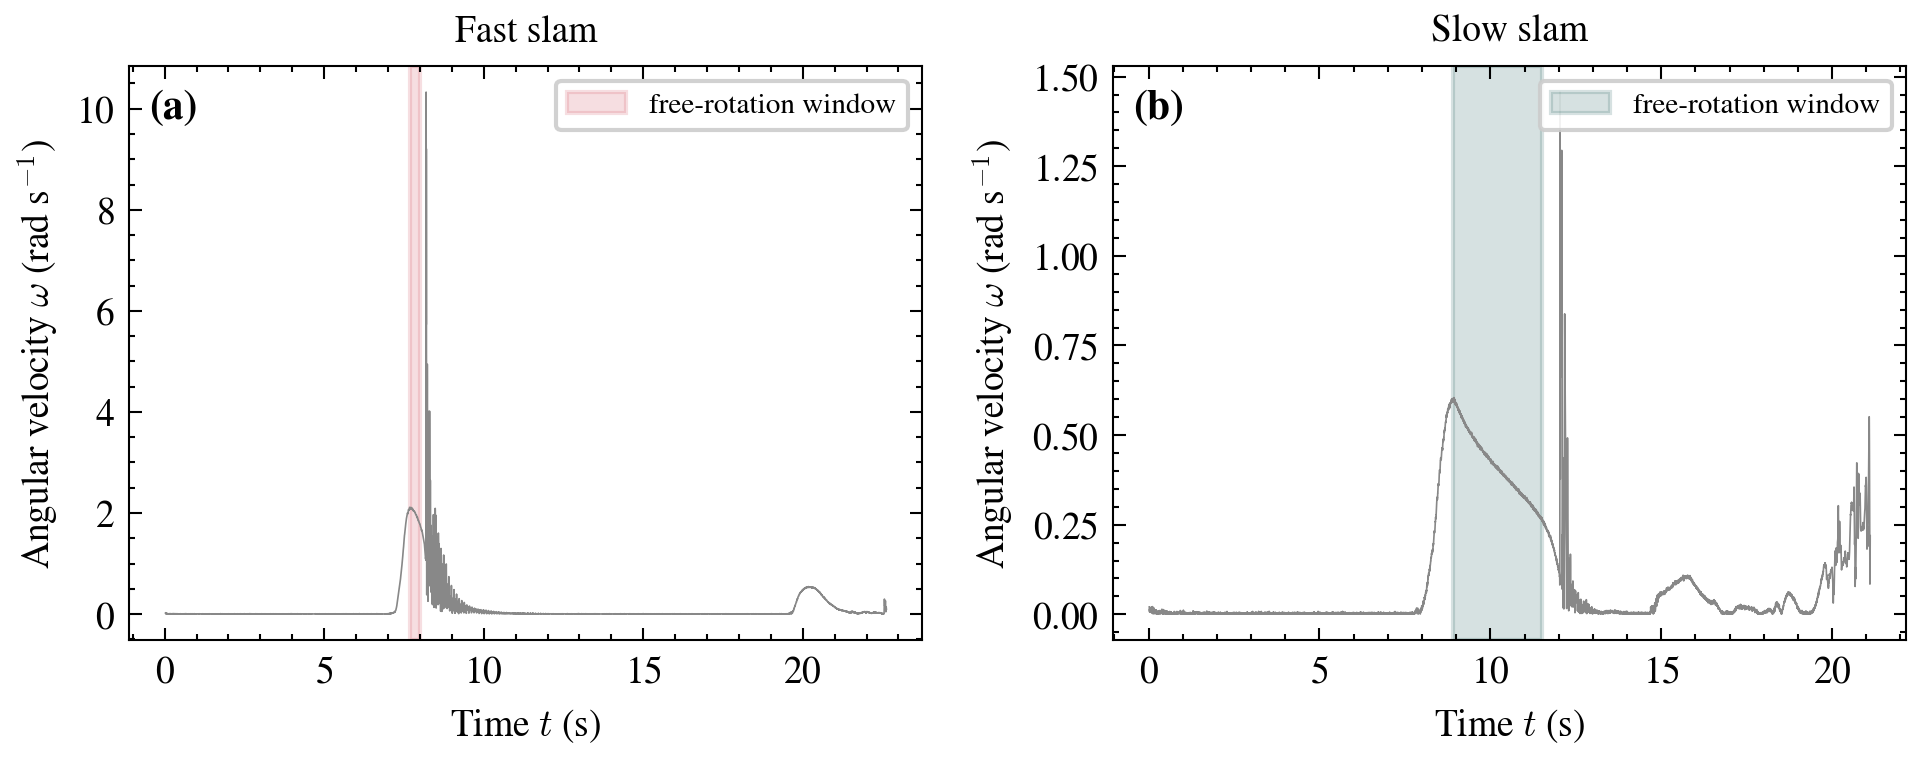
\includegraphics[width=\linewidth]{fig1_overview.png}
\caption{두 슬램의 자이로스코프 신호와 자유회전 분석 구간(음영). 날카로운 스파이크는 문틀과의
충돌로, 적합에서 제외하였다.}
\label{fig:overview}
\end{figure}

\subsection{6개 모델 적합}
각 모델을 \texttt{scipy.optimize.curve\_fit} 으로 적합하였다. 적합 파라미터와 적합도는
표~\ref{tab:fits_fast}, \ref{tab:fits_slow} 에, 적합 곡선은 그림~\ref{fig:fits} 에
나타냈다. 빠른 슬램에서는 각속도가 $2.08$ 에서 $1.79~\mathrm{rad/s}$ 까지, 즉
$0.86\,\omega_0$ 까지만 감소하며, 3절에서 예상한 대로 여섯 모델이 거의 똑같이 잘 맞는다
($R^2$ 는 $0.92$ 에서 $0.94$ 사이). 느린 슬램은 $0.60$ 에서 $0.27~\mathrm{rad/s}$ 로 더
넓은 범위를 가지며, 모델 간 차이가 드러난다. 건마찰 모델과 건마찰+뉴턴 모델을 비교한 내포
$F$-검정은 $F\approx4\times10^{3}$ ($p<0.001$) 을 주어, 순수 선형 법칙이 통계적으로
부적절하며 데이터가 곡률을 요구함을 보인다.

\begin{table}[h]\centering
\caption{적합 파라미터 및 적합도 --- 빠른 슬램.}
\label{tab:fits_fast}
\begin{tabular}{lcccccc}
\toprule
모델 & $a/I$ & $b/I$ & $c/I$ & $R^2$ & SSE & $\Delta$AIC \\
\midrule
\textbf{D} & 1.088 & -- & -- & 0.9441 & 0.08098 & 0.0 \\
S & -- & 0.5432 & -- & 0.9343 & 0.0952 & 23.3 \\
N & -- & -- & 0.2706 & 0.9238 & 0.1104 & 44.7 \\
DS & 1.088 & 1.923e-07 & -- & 0.9441 & 0.08098 & 2.0 \\
DN & 1.088 & -- & 4.58e-18 & 0.9441 & 0.08098 & 2.0 \\
SN & -- & 0.5432 & 1.78e-20 & 0.9343 & 0.0952 & 25.3 \\
\bottomrule
\end{tabular}
\end{table}

\begin{table}[h]\centering
\caption{적합 파라미터 및 적합도 --- 느린 슬램.}
\label{tab:fits_slow}
\begin{tabular}{lcccccc}
\toprule
모델 & $a/I$ & $b/I$ & $c/I$ & $R^2$ & SSE & $\Delta$AIC \\
\midrule
D & 0.1203 & -- & -- & 0.9879 & 0.12 & 1785.3 \\
S & -- & 0.2911 & -- & 0.9967 & 0.03321 & 236.5 \\
N & -- & -- & 0.6752 & 0.9896 & 0.103 & 1601.9 \\
DS & 0.0001393 & 0.2908 & -- & 0.9967 & 0.03321 & 238.5 \\
\textbf{DN} & 0.05793 & -- & 0.3556 & 0.9973 & 0.02725 & 0.0 \\
SN & -- & 0.2699 & 0.0495 & 0.9967 & 0.03277 & 222.4 \\
\bottomrule
\end{tabular}
\end{table}


\begin{figure}[h!]
\centering
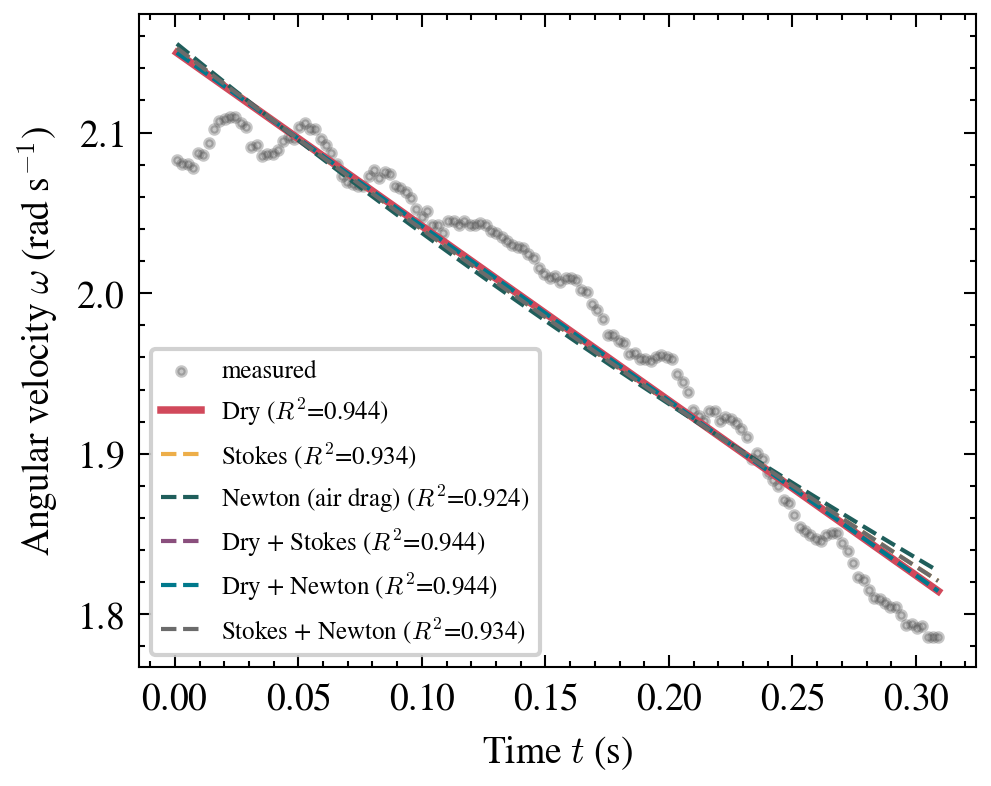
\includegraphics[width=0.49\linewidth]{fig_fit_fast.png}\hfill
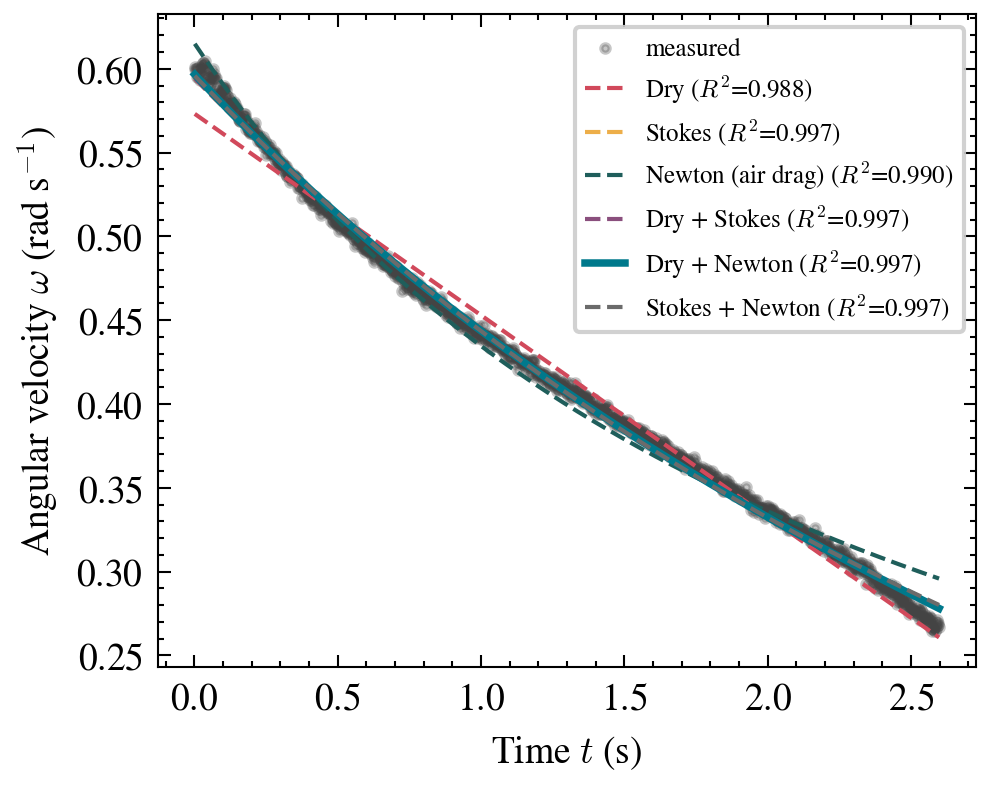
\includegraphics[width=0.49\linewidth]{fig_fit_slow.png}
\caption{빠른(왼쪽)·느린(오른쪽) 슬램의 자유회전 구간에 대한 6개 모델 적합. 느린 경우
직선인 건마찰 곡선이 데이터의 곡률을 명백히 벗어난다.}
\label{fig:fits}
\end{figure}

\subsection{해석해의 수치적 검증}
2절의 해석식이 옳은지 확인하기 위해, 적합 계수를 써서 식~\eqref{eq:ode} 을
\texttt{scipy.integrate.solve\_ivp} (RK45) 로 직접 적분하고 해석 곡선과 비교하였다
(그림~\ref{fig:sim}). 두 곡선은 약 $10^{-8}~\mathrm{rad/s}$ 수준에서 일치하며, 이는
수치적 반올림 오차 정도로 유도가 옳음을 확인해 준다. 같은 루틴은 간단한 닫힌 형태가 없는
일반 모델에도 적용된다.

\begin{figure}[h!]
\centering
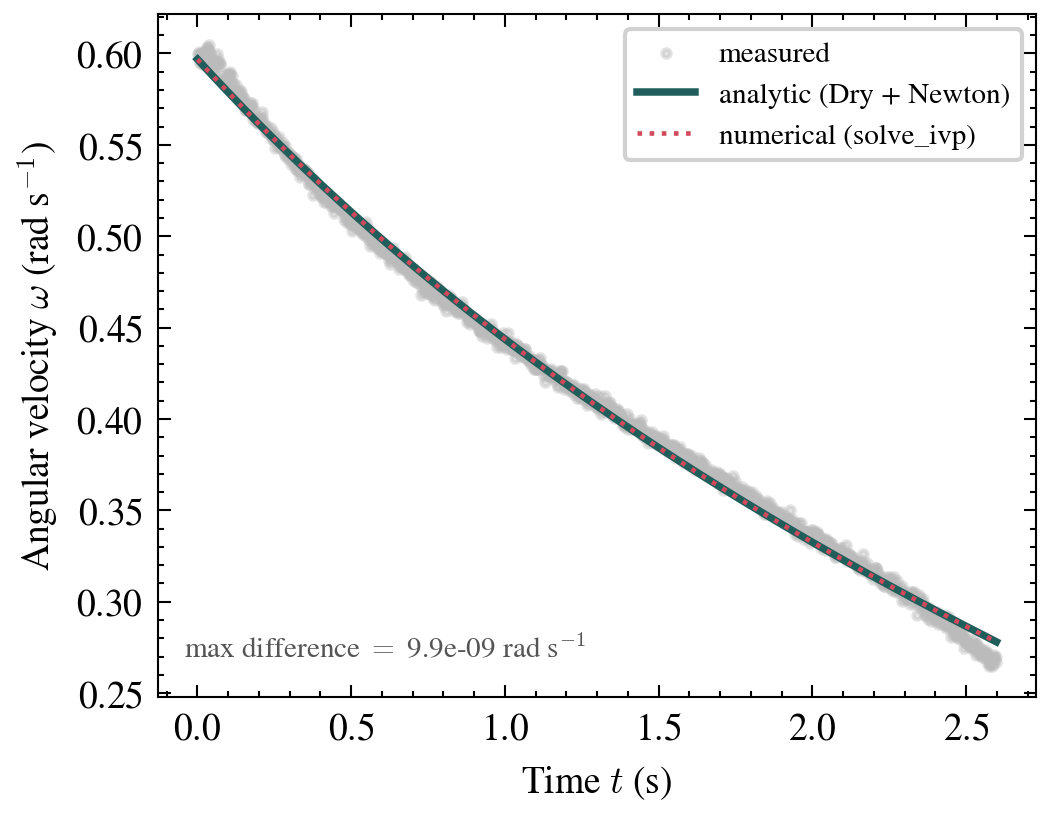
\includegraphics[width=0.66\linewidth]{fig4_simulation.png}
\caption{느린 슬램에 대한 해석해와 직접 수치적분의 비교. 두 곡선은 구별되지 않는다(최대 차이
$\sim10^{-8}$~rad/s).}
\label{fig:sim}
\end{figure}

% =========================================================================
\section{비판적 분석 및 논의}
% =========================================================================
적합도만으로는 모델을 선택할 수 없으므로, 원논문을 따라 각 적합 계수를 제1원리에서 얻은
차원 추정과 대조한다. 건마찰은 $a/I=3\mu g/w$, 스토크스 항력은
$b/I\lesssim 18\pi\eta w/m$, 뉴턴 항력은 $c/I\lesssim\tfrac32 C_D\rho A w/m$ 이며,
$\eta=1.7\times10^{-5}~\mathrm{Pa\,s}$, $\rho=1.3~\mathrm{kg/m^3}$, $C_D=1.5$ 를 쓴다.
비교 결과는 표~\ref{tab:validity} 와 그림~\ref{fig:validity} 에 정리하였다.

\begin{table}[h]\centering
\caption{적합 계수의 차원분석 타당성 (Klein et al. 참조).}
\label{tab:validity}
\begin{tabular}{llll}
\toprule
계수 & 적합값 (빠름 / 느림) & 이론 추정 & 판정 \\
\midrule
$a/I$ (건마찰) & 1.088 / 0.120 & $3\mu g/w$, $\mu$=0.031/0.0034 & 기각 ($\mu$ 9배 불일치) \\
$b/I$ (스토크스) & 0.543 / 0.291 & $\sim 6\times10^{-5}$ & 기각 ($10^3$--$10^4$배 과대) \\
$c/I$ (뉴턴) & 0.271 / 0.675 & $\lesssim 0.30$ & \textbf{채택 (같은 자릿수)} \\
\bottomrule
\end{tabular}
\end{table}


\begin{figure}[h!]
\centering
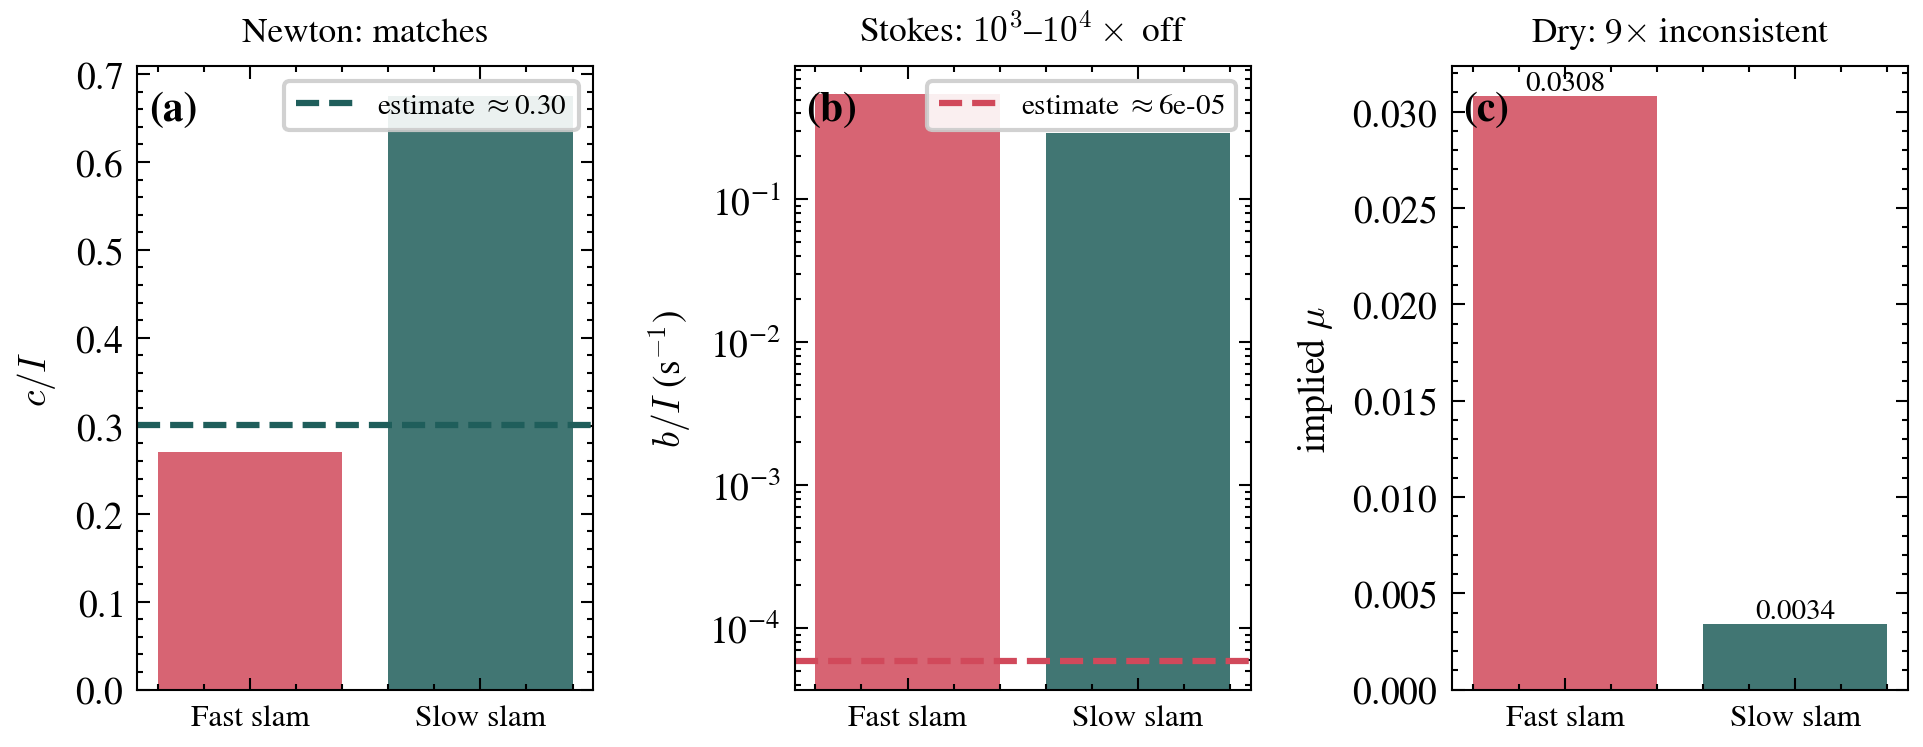
\includegraphics[width=\linewidth]{fig5_validity.png}
\caption{적합 계수와 물리적 추정의 대조. 뉴턴 $c/I$ 는 추정값에 거의 일치하고, 스토크스
$b/I$ 는 3{--}4 자릿수만큼 크며, 건마찰 계수는 양립 불가능한 두 $\mu$ 값을 함의한다.}
\label{fig:validity}
\end{figure}

적합된 스토크스 계수는 약 $0.3$ 에서 $0.6~\mathrm{s^{-1}}$ 로, 추정값
$6\times10^{-5}~\mathrm{s^{-1}}$ 의 대략 $10^{3}$ 에서 $10^{4}$ 배에 달한다. 따라서
스토크스 항력은 관측된 감속을 설명하기에 지나치게 약하다. 건마찰 모델은 함의된 미끄럼
마찰계수를 살펴보기 전까지는 적절해 보인다. 그 값은 빠른 슬램에서 $\mu\approx0.031$,
느린 슬램에서 $\mu\approx0.0034$ 로 9배나 차이 난다. $\mu$ 는 재료 상수여서 초기 각속도에
의존할 수 없으므로 건마찰 모델은 내적으로 모순된다. Klein 등도 함의된 토크가 비현실적으로
크다는 유사한 근거로 이를 기각하였다. 뉴턴 계수는 자신의 추정과 부합하는 유일한 항이다.
적합값 $c/I=0.27$(빠름)과 $0.68$(느림)은 추정값 $0.30$ 과 같은 자릿수이며, 낮은 각속도에서
$c/I$ 가 커지는 경향은 원논문이 보고한 추세를 재현한다. 원논문은 이를 항력계수 $C_D$ 의
레이놀즈 수 의존성으로 설명하였다.

측정의 한계도 밝혀 둔다. 빠른 슬램은 그 자체만으로는 모델을 구별하기에 너무 짧다.
슬램법의 이러한 한계는 원논문에도 보고되어 있는데, 거기서도 $\omega$ 는 충돌 전
$0.75\,\omega_0$ 정도까지만 감소한다. 이 짧고 노이즈가 큰 구간에서는 제약 없는 적합이
오히려 가장 단순한 건마찰 모델을 약간 선호하는데, 이는 3절에서 기술한 상황이며 물리적
타당성 검정으로 해소된다. Klein 등은 가벼운 판으로 더 긴 구간을 얻는 별도의 실험실 실험으로
이 문제를 피하였다. 본 연구의 자연스러운 확장은 문을 더 큰 각도에서 더 큰 각속도로 놓아
문틀에 닿지 않고 더 긴 호에 걸쳐 감속하도록 다시 측정하는 것이다. 그 밖의 불확실성 요인으로는
빠른 구간의 낮은 $R^2$ 로 나타나는 자이로스코프 노이즈, $r$ 의 불확실성, $I$ 에 대한 얇은
판 근사가 있다.

% =========================================================================
\section{결론}
% =========================================================================
스마트폰 자이로스코프로 실제 문을 측정하고, Klein 등의 마찰 모델을 중간 단계까지 채워
재구성하였으며, 해석해를 직접 수치적분으로 검증하였다. 여섯 모델 중 스토크스와 건마찰 항은
물리적 근거로 배제되는데, 전자는 계수의 3{--}4 자릿수 불일치 때문이고 후자는 시행 간에
일정하지 않은 계수 때문이다. 결국 2차 뉴턴 공기저항 항이 유일하게 물리적으로 타당한 기술로
남으며, 이는 원논문의 결론과 일치한다. 구체적 결과를 넘어, 본 프로젝트는 데이터와의 일치가
모델을 확립하기에 충분치 않으며 적합된 매개변수를 독립적인 물리적 추론과 대면시켜야 한다는
일반적 방법론적 교훈을 보여 준다.

\begin{thebibliography}{9}
\bibitem{klein2017} P.~Klein, A.~M\"uller, S.~Gr\"ober, A.~Molz, J.~Kuhn,
``Rotational and frictional dynamics of the slamming of a door,''
\textit{American Journal of Physics} \textbf{85}(1), 30--37 (2017).
\bibitem{repo} Team solvE, \textit{physics-door-slam}, 분석 코드 및 데이터,
\url{https://github.com/eeuunn/physics-door-slam}.
\end{thebibliography}
\end{document}
